\documentclass{beamer}
\usetheme{metropolis}

% Language packages
\usepackage[utf8]{inputenc}
\usepackage[T1]{fontenc}
\usepackage[portuguese]{babel}

% Code related packages/commands
\usepackage{caption}
\usepackage[newfloat]{minted}

\usepackage{hyperref}


\title{AMD Memory Encryption}
\author{João Gabriel Trombeta\\
        João Paulo Taylor Ienczak Zanette\\
        Ranieri Schroeder Althoff}
\date{\today}

\setbeamertemplate{footline}[page number]{}

\usepackage[font=scriptsize]{caption}
\newcommand{\source}[1]{\caption*{\tiny Retirado de: {#1}} }

\newcommand{\innertitle}[1]{\textbf{\large {#1}}}
\newcommand{\autotitle}[1]{\secname{} --- \subsecname}

\begin{document}

\maketitle{}

\section{Máquinas Virtuais}

\subsection{Definições}

\begin{frame}{\secname{} --- \subsecname}
    \innertitle{Máquina Virtual (VM)}

    Emuladores de computadores lógicos.
    \begin{description}
        \item[\textit{Guest}:] O computador executado pela VM\@;
        \item[\textit{Host}:] Computador que oferece recursos para a VM\@.
    \end{description}
\end{frame}

\begin{frame}{\secname{} --- \subsecname}
    \innertitle{Hypervisor}

    ``Monitor de Máquina Virtual'': cria, executa e gerencia uma ou mais VMs\@.

    \begin{description}
        \item[\textit{Bare Metal}:] quando executa a VM diretamente no
            \textit{hardware}.
        \item[\textit{Hosted}:] quando executa \textit{software} sobre o SO do
            \textit{Host}.
    \end{description}

    \begin{figure}[h]
        \centering
        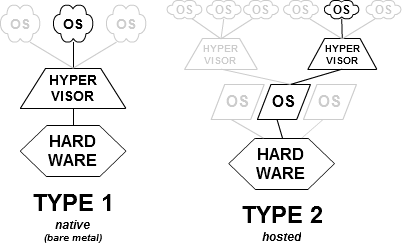
\includegraphics[keepaspectratio,width=.5\textwidth]{img/hypervisor}
        \source{\url{https://en.wikipedia.org/wiki/Hypervisor}}
    \end{figure}
\end{frame}

\section{Falhas em Hypervisors}

\subsection{Xen Hypervisor}

\begin{frame}{\secname{} --- \subsecname}
    \innertitle{Xen Hypervisor}

    \begin{itemize}
        \item Um dos \textit{Hypervisors} mais populares atualmente;
        \item \textit{Bare-Metal};
        \item \textit{Open-Source}.
    \end{itemize}

    \begin{figure}
        
\includegraphics[keepaspectratio,height=.3\textheight]{img/xen-panda}
        \source{\url{http://www-archive.xenproject.org/products/xenhyp.html}}
    \end{figure}
\end{frame}

\begin{frame}{\secname{} --- \subsecname}
    \innertitle{Descrição da falha}

    \begin{itemize}
        \item Conforme descrito em~\cite{xen-exploit}, é possível fazer
            leitura/escrita de código arbitrário no espaço de endereçamento do
            \textit{Guest};
        \item Descobrindo a localização da \textbf{tabela de hypercall}, é
            possível executar uma rotina como \textit{Host} (fazendo
            \textbf{escape de máquina virtual}).
    \end{itemize}
\end{frame}

\begin{frame}[fragile]{\secname{} --- \subsecname}
    \innertitle{Tabela de \textit{Hypercall}}

    \inputminted[fontsize=\scriptsize]{asm}{hypercall-table.S}
\end{frame}

\begin{frame}{\autotitle{}}
    \innertitle{Procedimento para explorar a falha}

    \begin{enumerate}
        \item Criar a situação de acesso irrestrito à memória do
            \textit{Guest};
        \item Varrer as páginas do \textit{Guest}, fazendo \textit{checksum} do
            conteúdo de cada uma;
        \item Localizar a tabela de \textit{hypercall} através da tabela de
            argumentos de \textit{hypercall}.
        \item Sobrescrever o endereço de um dos \textit{hypercalls} para uma
            rotina maliciosa;
        \item Ativar o evento para o \textit{hypercall} alterado.
    \end{enumerate}
\end{frame}

\section{AMD Memory Encryption}

\subsection{Sobre}

\begin{frame}{\autotitle{}}
    \innertitle{Motivação}

    Tornar mais seguro o uso de máquinas virtuais através do Secure Memory
    Encryption (SME) e Secure Encrypted Virtualization (SEV).
\end{frame}

\subsection{AMD Secure Processor}

\begin{frame}{\autotitle{}}
    \innertitle{\subsecname}

    Processador dedicado à criptografia.

    \begin{itemize}
        \item Antigo PSP (Platform Security Processor);
        \item Independente;
        \item Executa um \textit{kernel} confiável e de código fechado;
        \item Isola procedimentos de segurança;
        \item Memória dedicada;
        \item Acesso ao CCP (Coprocessador criptográfico).
    \end{itemize}

    \begin{figure}
        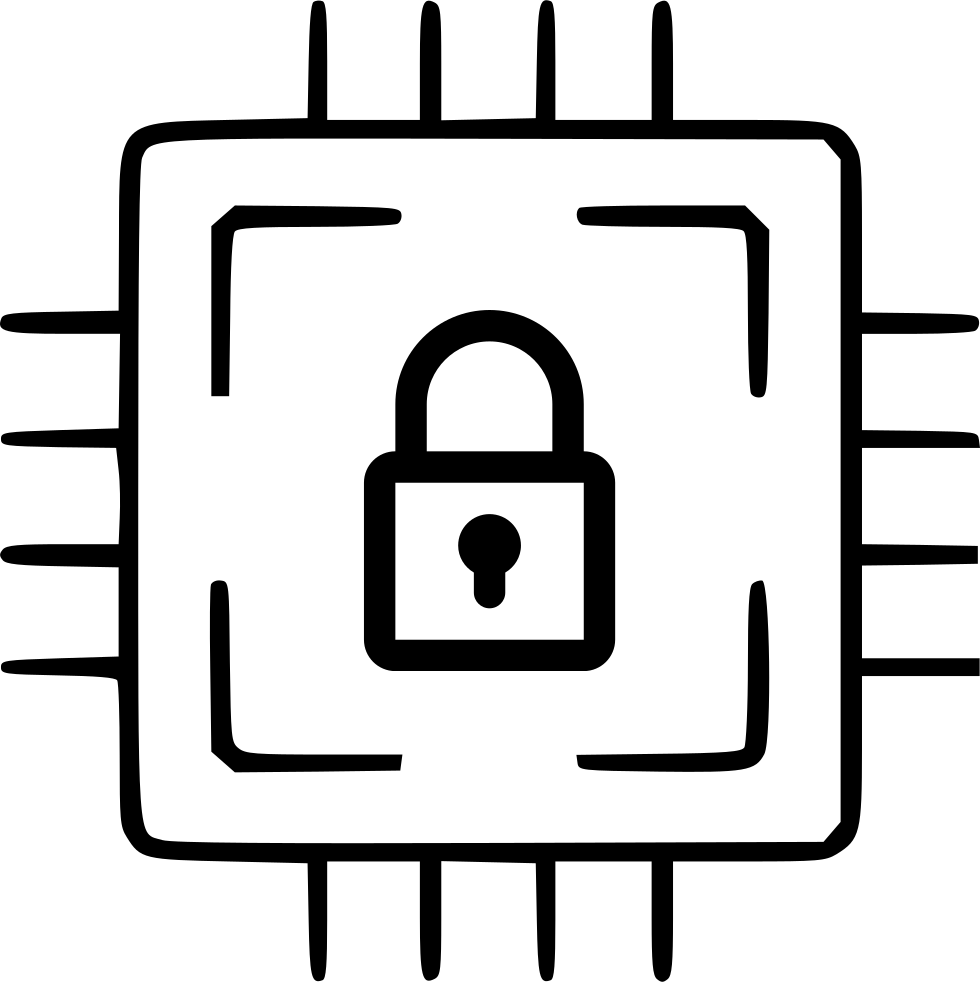
\includegraphics[keepaspectratio,height=4em]{img/crypto-proc}
    \end{figure}
\end{frame}

\subsection{Security Memory Encryption}

\begin{frame}{\autotitle{}}
    \innertitle{\subsecname}

    \begin{itemize}
        \item Criptografa e descriptografa dados escritos na RAM\@;
        \item Utiliza uma única chave simétrica;
        \item \textit{Engine} de criptografia \textit{On-chip};
        \item Criptografia entre SO/\textit{hypervisor} e RAM\@;
    \end{itemize}
\end{frame}

\begin{frame}{\autotitle{}}
    \begin{figure}
        \centering
        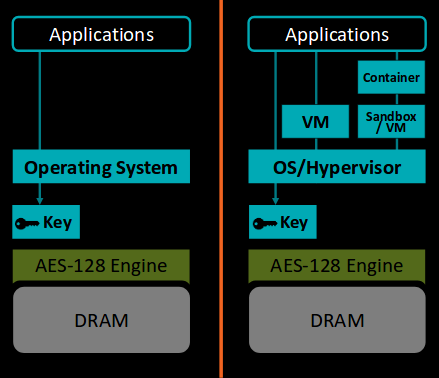
\includegraphics[keepaspectratio,height=.8\textheight]{img/sme}
        \caption{Método de criptografia do SME.}
    \end{figure}
\end{frame}

\begin{frame}{\autotitle{}}
    \innertitle{Requisitos}

    \begin{itemize}
        \item Suporte em \textit{hardware} por parte do processador
            (verificável pela chamada de CPUID Fn8000\_001F);
        \item Habilitar o recurso deixando o bit 23 do MSR (Model-Specific
            Register) em 1;
        \item O último bit mais significativo dos endereços (C-Bit) passa a
            sinalizar se o dado deve ou não ser criptografado/descriptografado.
    \end{itemize}
\end{frame}

\begin{frame}{\autotitle{}}
    \begin{figure}
        \centering
        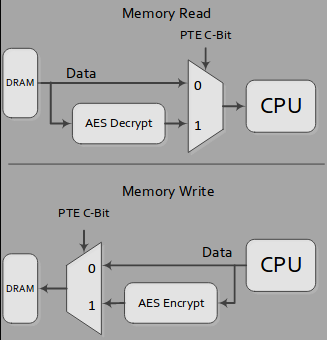
\includegraphics[keepaspectratio,height=.8\textheight]{img/sme_read_write_architecture}
        \caption{Leitura e escrita no SME.}
    \end{figure}
\end{frame}

\begin{frame}{\autotitle{}}
    \innertitle{Transparent SME}

    Variação do SME em que tudo é criptografado.

    \begin{itemize}
        \item Não necessita suporte pelo SO\@.
    \end{itemize}
\end{frame}

\subsection{Secure Encrypted Virtualization}

\begin{frame}{\autotitle{}}
    \innertitle{\subsecname}

    Integra o SME com a capacidade de comportar várias VMs criptografadas.

    \begin{itemize}
        \item \textit{Host} possui uma chave;
        \item Cada VM possui uma chave própria;
        \item Cada VM é protegida separadamente.
    \end{itemize}
\end{frame}

\begin{frame}{\autotitle{}}
    \begin{figure}
        \centering
        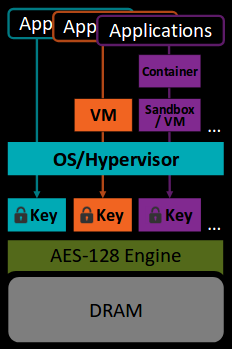
\includegraphics[keepaspectratio,height=.8\textheight]{img/sev}
        \caption{Demonstração do acesso á memória através de chaves.}
    \end{figure}
\end{frame}

\begin{frame}{\autotitle{}}
    \begin{figure}
        \centering
        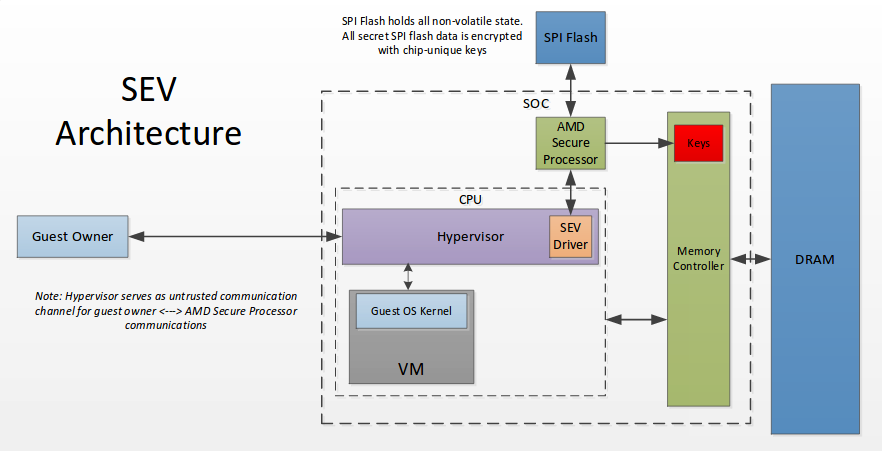
\includegraphics[keepaspectratio,width=1\textwidth]{img/sev-architecture}
        \caption{Visão geral da arquitetura do SEV.}
    \end{figure}
\end{frame}

\begin{frame}{\autotitle{}}
    \innertitle{Address Space ID}

    Identifica qual chave pertence a qual VM\@.

    \begin{itemize}
        \item Utilizado como parte do endereço para \textit{tag} na TLB\@;
        \item Auxilia na eficiência permitindo que dados de mais de uma VM
            permaneça na TLB ao mesmo tempo.
    \end{itemize}

    \begin{figure}
        \centering
        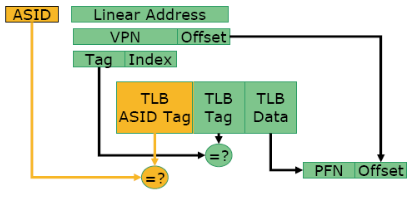
\includegraphics[keepaspectratio,height=.4\textheight]{img/asid}
        \caption{Comportamento da TLB mediante ASID\@.}
    \end{figure}
\end{frame}

\begin{frame}{\autotitle{}}
    \begin{figure}
        \centering
        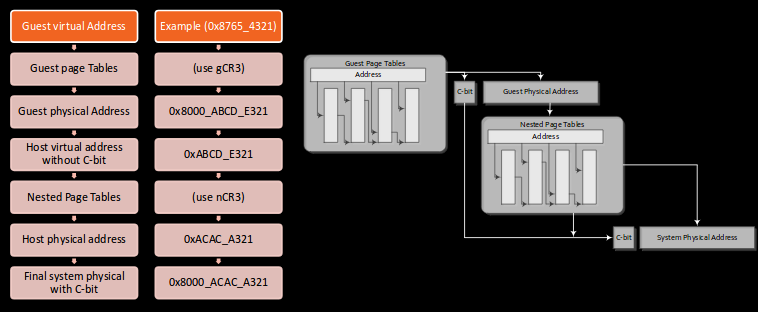
\includegraphics[keepaspectratio,width=1\textwidth]{img/sev-address-translation}
        \caption{Tradução de endereços do SEV\@.}
    \end{figure}
\end{frame}

\begin{frame}{\autotitle{}}
    \innertitle{Conflito de criptografia}

    Pode ocorrer de o \textit{Host} e o \textit{Guest} tentarem criptografar a
    mesma página. Nesse caso, a preferência é utilizar a chave do
    \textit{Guest}.
\end{frame}

\begin{frame}{\autotitle{}}
    \innertitle{Proteção contra falha de segurança}

    SEV pode oferecer proteção contra a falha apresentada no Xen Hypervisor:

    \begin{enumerate}
        \item Os \textit{Checksums} serão feitos por um \textit{Guest} com
            acesso irrestrito de leitura/escrita em sua memória;
        \item As leituras das páginas serão descriptografadas usando a chave do
            \textit{Guest};
        \item A região das \textit{hypercalls} está criptografada usando a
            chave do \textit{Host};
        \item Logo, as leituras das \textit{hypercalls} será feita erroneamente
            e portanto não serão identificadas pela assinatura esperada.
    \end{enumerate}
\end{frame}

\section{Utilização do SME e SEV}

\subsection{Execução de comandos}

\begin{frame}{\autotitle{}}
    \innertitle{\textit{Set-up}}

    \begin{enumerate}
        \item Comandos são efetuados pelo \textit{Command buffer};
        \item Endereço do \textit{Command buffer} precisa ser definido nos
            registradores \texttt{CmdBufAddr\_\{Hi,Lo\}};
        \item O \textit{Driver} altera o \textit{Command buffer} habilitando os
            campos de bits necessários para descrição do comando;
        \item O AMD-SP executa o comando;
        \item \textit{Command buffer} é atualizado com a resposta do comando.
    \end{enumerate}
\end{frame}

\begin{frame}{\autotitle{}}
    \innertitle{Emissão de um comando}

    \scriptsize\texttt{\begin{center}
        \begin{tabular}{|c|c|c|c|c|}
            \hline
            31 & 30--26 & 25--16 & 15--1 & 0 \\
            \hline
            0  & ---    & ID     & ---   & IR \\
            \hline
        \end{tabular}
    \end{center}}

    \begin{description}
        \item[ID:] ID do comando a ser emitido;
        \item[IR:] Habilitar interrupções ao finalizar comando.
    \end{description}

    \innertitle{Resposta da AMD-SP}

    \scriptsize\texttt{\begin{center}
        \begin{tabular}{|c|c|c|}
            \hline
            31 & 30--16 & 15--0 \\
            \hline
            1  & ---    & ST \\
            \hline
        \end{tabular}
    \end{center}}

    \begin{description}
        \item[ST:] Código de status.
    \end{description}
\end{frame}

\begin{frame}{\autotitle{}}
    \innertitle{Comandos}

    \begin{itemize}
        \item INIT\@;
        \item SHUTDOWN\@;
        \item PLATFORM\_RESET\@;
        \item PLATFORM\_STATUS\@;
        \item PEK\_GEN\@;
        \item PEK\_CSR\@;
        \item PEK\_CERT\_IMPORT\@;
        \item PDH\_GEN\@;
        \item PDH\_CERT\_EXPORT\@.
    \end{itemize}
\end{frame}

\begin{frame}{\autotitle{}}
    \tiny{\begin{table}[h]
    \centering
    \begin{tabular}{lll}
        \toprule
        Status  & Código\\
        \midrule
        SUCCESS & 0000h\\
        INVALID\_PLATFORM\_STATE & 0001h\\
        INVALID\_GUEST\_STATE & 0002h\\
        INVALID\_CONFIG & 0003h\\
        INVALID\_LENGTH & 0004h\\
        ALREADY\_OWNED & 0005h\\
        INVALID\_CERTIFICATE & 0006h\\
        POLICY\_FAILURE & 0007h\\
        INACTIVE & 0008h\\
        INVALID\_ADDRESS & 0009h\\
        BAD\_SIGNATURE & 000Ah\\
        BAD\_MEASUREMENT & 000Bh\\
        ASID\_OWNED & 000Ch\\
        INVALID\_ASID & 000Dh\\
        WBINVD\_REQUIRED & 000Eh\\
        DFFLUSH\_REQUIRED & 0009h\\
        INVALID\_GUEST & 0010h\\
        INVALID\_COMMAND & 0011h\\
        ACTIVE & 0012h\\
        HWERROR\_PLATFORM & 0013h\\
        HWERROR\_UNSAFE & 0014h\\
        UNSUPPORTED & 0015h\\
        INVALID\_PARAM & 0016h\\
        \bottomrule
    \end{tabular}
    \caption{Relação dos códigos de status dados pelo AMD-SP\@. Mais detalhes
             sobre a tabela estão
             em~\cite{sev-api-doc}}\label{cmdresp-status-code}
\end{table}

}
\end{frame}

\section{Comentários finais}

\subsection{Possíveis falhas}

\begin{frame}{\autotitle{}}
    \innertitle{\subsecname}

    Apesar dos esforços, a implementação atual do SEV ainda possui falhas de
    segurança.

    \begin{itemize}
        \item A mesma chave fica associada a uma VM durante toda a existência
            dela;
        \item A implementação de \textit{Nested Pages} pode ser explorada para
            trocar informações entre \textit{Guests} aproveitando que o
            \textit{Host} consegue descriptografá-los.
    \end{itemize}
\end{frame}

\bibliographystyle{ieeetr}

\begin{frame}{Referências}
    \nocite{*}
    \bibliography{references}
\end{frame}

\end{document}
